\documentclass{article}
\usepackage{graphicx}
\usepackage{hyperref}
\usepackage{xcolor}
% Here: H option for float placement
\usepackage{float}

% caption and subcaption work together
\usepackage{subcaption} % loads the caption package

\graphicspath{ {images/} }

\begin{document}
\pagecolor{white}

\title{%
  Multi-class Weather Image classifier
  \large \\HW2 - ML Sapienza}

\author{Giulio Serra 1904089}
\date{December 15, 2019}

\maketitle


\begin{titlepage}
\end{titlepage}

\tableofcontents

\begin{titlepage}
\end{titlepage}


\section{Introduction}\label{sec:intro}
This essay will describe the implementation of a multi-class image classifier using Pyton with the Tensorflow library.

\section{The image classification Problem}
The aim of this implementation is to train a learning algorithm based on neural network, to recognize the weather condition displayed on a set of images based upon four categories: 'HAZE', 'RAINY', 'SNOWY' and 'SUNNY'.\\
The problem is an instance of a multi class image classifier: the classification can be achieved by training a model using a neural network(NN for short).\\

\section{Neural Networks}
A neural network is a network supporting learning inspired by (but no identical to) the biological neural network.\\Models based on on neural networks can be trained by providing them examples that have been already labled to a specific category: then the model is able to extract some features from the examples to train itself.\\
Neural networks are build upon layers , the input layer contains the date while the hidden layer compute the learning process by extracting features from the raw data provided, for example, in the image recognition problem, every layer can have the task to recognize different features of the face (nose, eyes ecc..), in the end, the output layer output data in one of n nodes based on the features detected by previous layers. 

\begin{figure}[h] 
		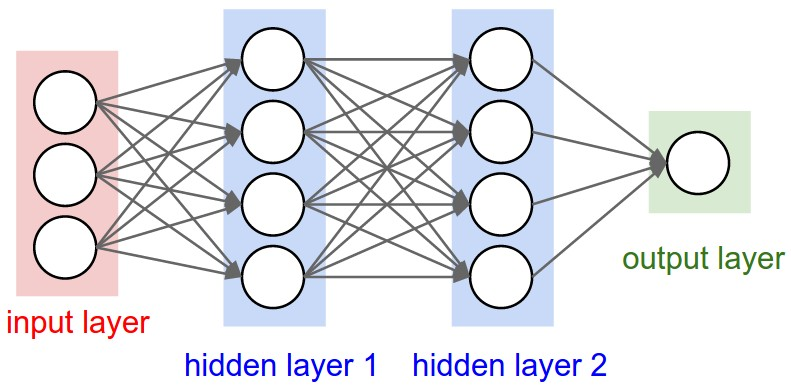
\includegraphics[width=0.8\textwidth ]{images/neural.jpg}
		\centering
		\caption{A small example of a neural network}
\end{figure}
 
 \subsection{Convolution Neural Network}
 A particular kind of neural network, (very well suited for image recognition), is the convolution neural network(CNN for short): while mantaing the typical layers of a neural network, the hidden layers consist of a series of mathematical operations of convolutions using matrixes(at least on one of the layers).\\
CNN are a regularized version of multilayer perceptrons(fully connected networks), they take advantage of the hierarchical pattern in data and assemble more complex patterns using simpler ones.When applied to image recognition, CNN learns to categorize images with the following steps:\\

\begin{figure}[h] 
		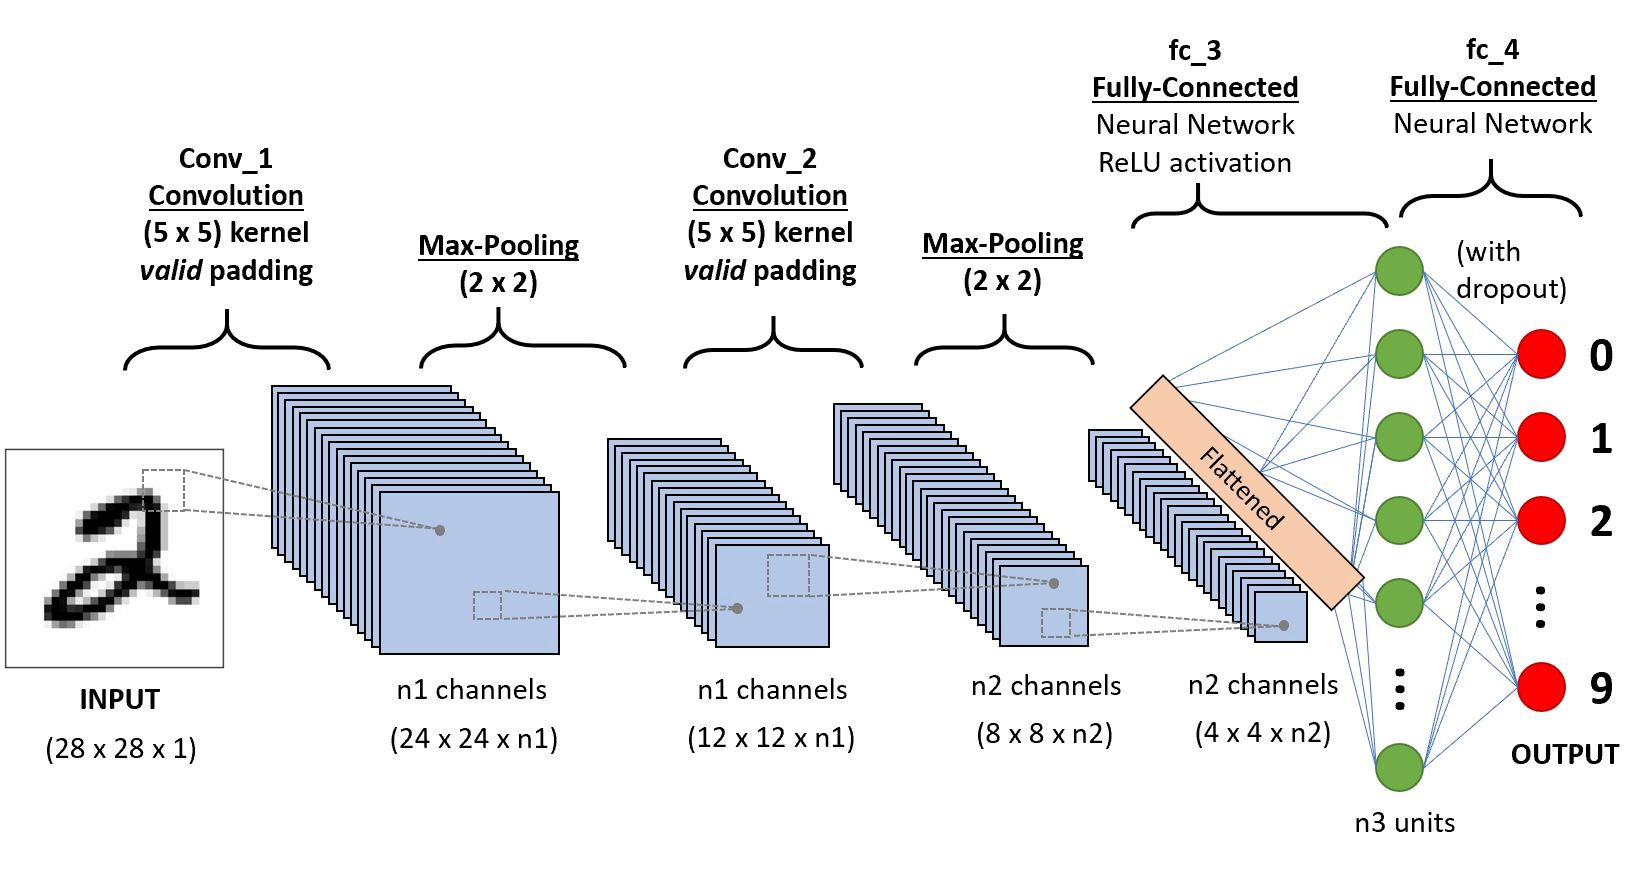
\includegraphics[width=0.8\textwidth ]{images/convolution.jpeg}
		\centering
		\caption{The Convolution Neural Network learning process}
\end{figure}

\begin{itemize}
 \item \textbf{Input Image}\\\\
 	Every image is decomposed to a 3x3xN(usually 4) matrix rappresenting the red, green and blue(RGB) value of every pixel, this task can be very resource-consuming for high resolution images, so to speed up the training process, every image need to be resized but without loosing any key information.
	
	\item \textbf{Convolution Layer — The Kernel}\\\\
	The first convolution operation is done between the matrix of the RGB value of the image and a Kernel filter, for example:
	
	\begin{verbatim}
	1  0  1
	0  1  0
	1  0  1
	\end{verbatim}
	
	The first layer of convolution aim to extract low-level features such as colors and shapes, while the upper layers extract-some high level features.
	
	\item \textbf{Pooling Layer}\\\\
	The Pooling layer is responsible for reducing the spatial size of the Convolved Feature. This is to decrease the computational power required to process the data, it is useful for extracting dominant features 		 thus maintaining the process of effectively training of the model.\\
	There are two types of Pooling: Max Pooling and Average Pooling: while the first one returns the maximum value from the portion of the image covered by the Kernel, Average Pooling returns the 	average of all the values from the portion of the image covered by the Kernel,
	Max Pooling also performs as a Noise Suppressant,it discards the noisy activations altogether and also performs de-noising along with dimensionality reduction. 

	\end{itemize}
	
\subsection{AlexNet}
	
A very effective type of convolution network is the AlexNet: it's designed around 8 layers: the first five are convolutional layers (some of them followed by max-pooling layers) and the last three are fully connected layers, here follows the implementation in Python using the Tensorflow library:

\begin{verbatim}
def AlexNet(input_shape, num_classes, regl2 = 0.0001, lr=0.0001):
    
    model = Sequential()

    # C1 Convolutional Layer 
    model.add(Conv2D(filters=96, input_shape=input_shape, kernel_size=(11,11),\
                     strides=(2,4), padding='valid'))
    model.add(Activation('relu'))
    # Pooling
    model.add(MaxPooling2D(pool_size=(2,2), strides=(2,2), padding='valid'))
    # Batch Normalisation before passing it to the next layer
    model.add(BatchNormalization())

    # C2 Convolutional Layer
    model.add(Conv2D(filters=256, kernel_size=(11,11), strides=(1,1), padding='valid'))
    model.add(Activation('relu'))
    # Pooling
    model.add(MaxPooling2D(pool_size=(2,2), strides=(2,2), padding='valid'))
    # Batch Normalisation
    model.add(BatchNormalization())

  .... other layers ....

    # Flatten
    model.add(Flatten())

    flatten_shape = (input_shape[0]*input_shape[1]*input_shape[2],)
    
    # D1 Dense Layer
    model.add(Dense(4096, input_shape=flatten_shape, kernel_regularizer=regularizers.l2(regl2)))
    model.add(Activation('relu'))
    # Dropout
    model.add(Dropout(0.4))
    # Batch Normalisation
    model.add(BatchNormalization())

   .. three dense layer...
   
    # Output Layer
    model.add(Dense(num_classes))
    model.add(Activation('softmax'))

    # Compile

    adam = optimizers.Adam(lr=lr)
    model.compile(loss='categorical_crossentropy', optimizer=adam, metrics=['accuracy'])

    return model
 
# create the model
model = AlexNet(inputShape,classes)
model.summary()
\end{verbatim}

 \section{Implementation}
 
 \subsection{Dataset Preparation}
 Since we are talking about image recognition, in order to better train our model, we need to uniform all the images to the same resolution/orientation:
 
 \begin{verbatim}
batch_size = 32

trainDatagen = ImageDataGenerator(
    rescale = 1. / 255,\
    zoom_range=0.1,\
    rotation_range=10,\
    width_shift_range=0.1,\
    height_shift_range=0.1,\
    horizontal_flip=True,\
    vertical_flip=False)

....

validationDatagen = ImageDataGenerator(
    rescale = 1. / 255,\
    zoom_range=0.1,\
    rotation_range=10,\
    width_shift_range=0.1,\
    height_shift_range=0.1,\
    horizontal_flip=True,\
    vertical_flip=False)

validationGenerator = testDatagen.flow_from_directory(
    directory=testSet,
    target_size=(256, 256),
    color_mode="rgb",
    batch_size=batch_size,
    class_mode="categorical",
    shuffle=False
)

 \end{verbatim}

\subsection{Results of AlexNet}

To evaluate the performances of a model we can use the classification report along the accuracy-epoch curve, here is the output of the AlexNet:

\begin{verbatim}
           precision    recall  f1-score   support

        HAZE      0.828     0.960     0.889       100
       RAINY      0.952     0.790     0.863       100
       SNOWY      0.850     0.910     0.879       100
       SUNNY      1.000     0.940     0.969       100

    accuracy                          0.900       400
   macro avg      0.907     0.900     0.900       400
weighted avg      0.907     0.900     0.900       400

True                 Predicted         	errors 	err % 
------------------------------------------------------------------
RAINY            ->  SNOWY             	13 	3.25 % 
SNOWY            ->  HAZE              	9 	2.25 % 
RAINY            ->  HAZE              	8 	2.00 % 
SUNNY            ->  HAZE              	3 	0.75 % 
HAZE             ->  RAINY             	2 	0.50 % 
HAZE             ->  SNOWY             	2 	0.50 % 
SUNNY            ->  RAINY             	2 	0.50 % 
SUNNY            ->  SNOWY             	1 	0.25 % 

\end{verbatim}


The accuracy-epoch curve shows how the model accuracy increase over every usage of the training vector to update the weights(epoch), while the loss-epoch curve show how the loss decrease(hopefully) for every iteration,here is the output of the AlexNet curves:

\begin{figure}[h]
\centering
\subcaptionbox{Accuracy curve}{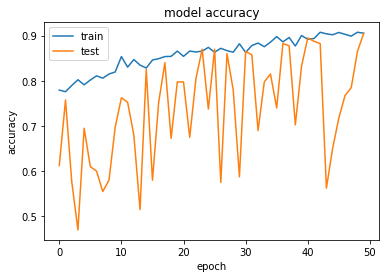
\includegraphics[width=0.5\textwidth]{images/accuracy.png}}%
\hfill % <-- Seperation
\subcaptionbox{Loss curve}{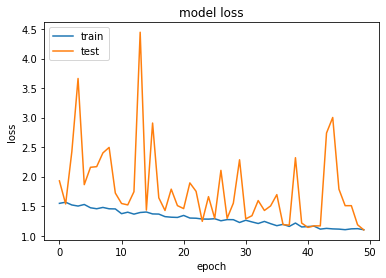
\includegraphics[width=0.5\textwidth]{images/loss.png}}%
\caption{AlexNet Results}
\end{figure}

While the accuracy of the Training Set increase and the loss decrease for every epoch, the Validation Set results are very poor: even with the normalization.\\
The gap between the Train Set curve and the Validation Set curve also measure how much our model is prone to overfitting(the model adapt too much on the data  in the trainSet while performing poor on the overall data available).\\\\
The last step before exporting our model is to compute the results on the test set (as a part of cross-validation procedure), here is the report matrix of AlexNet model over the test set:

\begin{verbatim}

        HAZE      0.817     0.940     0.874       100
       RAINY      0.955     0.840     0.894       100
       SNOWY      0.838     0.880     0.859       100
       SUNNY      1.000     0.920     0.958       100

    accuracy                          0.895       400
   macro avg      0.903     0.895     0.896       400
weighted avg      0.903     0.895     0.896       400

True                 Predicted         	errors 	err % 
------------------------------------------------------------------
RAINY            ->  SNOWY             	10 	2.50 % 
SNOWY            ->  HAZE              	10 	2.50 % 
RAINY            ->  HAZE              	6 	1.50 % 
SUNNY            ->  HAZE              	5 	1.25 % 
HAZE             ->  SNOWY             	4 	1.00 % 
SUNNY            ->  SNOWY             	3 	0.75 % 
HAZE             ->  RAINY             	2 	0.50 % 
SNOWY            ->  RAINY             	2 	0.50 %

\end{verbatim}

\section{ResNet}

\subsection{Model Selection}
In order to add layers to a model, we need to first choose an already trained model: the Tensorflow library provides the ResNet CNN architecture to enrich with new layers.\\
ResNet is designed to perform better with additional layers because it can process smaller features, so consequently, the training error decrease as the network gets deeper.\\
The first things to do it's to download the model and store it in a variable:\\

\begin{verbatim}
model = Sequential()
  resNet = tensorflow.keras.applications.resnet_v2.ResNet152V2(weights="imagenet",
  include_top=False,input_shape=inputShape)

  for layer in resNet.layers:
    if(layer == resNet.layers[-1] or layer == resNet.layers[-2]):
      layer.trainable=True
    else:
      layer.trainable=False
  
\end{verbatim}
We can actually choose how many layers to train, for the sake of computational power we can train just two more, in addition we can specify how many epochs to chose(in this case 50).\\
As usual we need to pass the TrainingSet and the ValidationSet to train our model:

\begin{verbatim}
for layer in resNet.layers:
    if(layer == resNet.layers[-1] or layer == resNet.layers[-2]):
      layer.trainable=True
    else:
      layer.trainable=False
  
  model.add(resNet)
  model.add(GlobalAveragePooling2D()) #MINOR Overfitting

  model.add(Dense(512,activation = "relu"))
  model.add(BatchNormalization()) #Normalization
  model.add(Dropout(0.25))

  model.add(Dense(64,activation = "relu"))
  model.add(Dropout(0.25))

  model.add(Dense(64,activation = "relu"))
  model.add(Dropout(0.25))

  model.add(Dense(num_classes))
  model.add(Activation('softmax'))
  model.compile(optimizer=Adam(lr=0.0001),loss='categorical_crossentropy',
  metrics=['accuracy'])
  return model
  ...
trained.compile(optimizer='Adam',loss='categorical_crossentropy',metrics=['accuracy'])

steps_per_epoch=trainGenerator.n//trainGenerator.batch_size
val_steps=validationGenerator.n//validationGenerator.batch_size+1

print(steps_per_epoch)
print(val_steps)

history = trained.fit_generator(trainGenerator, epochs=50, verbose=1,\
                    steps_per_epoch=steps_per_epoch,\
                    validation_data=validationGenerator,\
                    validation_steps=val_steps)

\end{verbatim}

\subsection{Results}
To evaluate the results we use the same parameters as before: the report matrix along the accuracy and loss curves:

\begin{verbatim}
              precision    recall  f1-score   support

        HAZE      0.857     0.960     0.906       100
       RAINY      1.000     0.890     0.942       100
       SNOWY      0.914     0.960     0.937       100
       SUNNY      0.979     0.920     0.948       100

    accuracy                          0.932       400
   macro avg      0.938     0.932     0.933       400
weighted avg      0.938     0.932     0.933       400

True                 Predicted         	errors 	err % 
------------------------------------------------------------------
RAINY            ->  HAZE              	7 	1.75 % 
SUNNY            ->  HAZE              	5 	1.25 % 
HAZE             ->  SNOWY             	4 	1.00 % 
SNOWY            ->  HAZE              	4 	1.00 % 
SUNNY            ->  SNOWY             	3 	0.75 % 
RAINY            ->  SNOWY             	2 	0.50 % 
RAINY            ->  SUNNY             	2 	0.50 % 
\end{verbatim}

Here follows the accuracy and loss curves:

\begin{figure}[h]
\centering
\subcaptionbox{Accuracy curve}{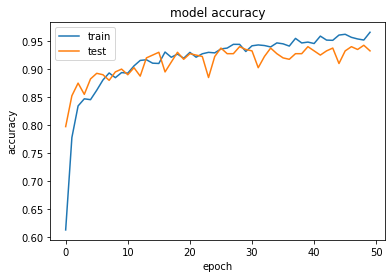
\includegraphics[width=0.5\textwidth]{images/ResNet_accuracy.png}}%
\hfill % <-- Seperation
\subcaptionbox{Loss curve}{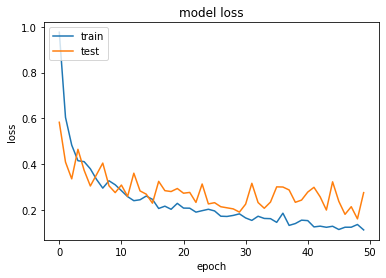
\includegraphics[width=0.5\textwidth]{images/ResNet_loss.png}}%
\caption{ResNet Results}
\end{figure}

The performances are way better than the previous model(AlexNet) as highlighted by the training curve,(that closely follows the train curve), also the space between the two curves is very small meaning there is little to no overfitting.

\clearpage
\section{BlindTest Validation}

The final step to validate our model is to feed it with the BlindTest, so first we need to import the best model(in term of performances), in this case we chose the ResNet model:

\begin{verbatim}
try:
  model = load_model(datadir + 'models/TRAINED_MODEL.h5')
  print('Model loaded sucessfully')
except OSError:
  print('Model loaded sucessfully')
\end{verbatim}
Then we need to provide the model with the Blind Set:

\begin{verbatim}
batch_size = 32

blindDatagen = ImageDataGenerator(
    rescale = 1. / 255,\
    zoom_range=0.1,\
    rotation_range=10,\
    width_shift_range=0.1,\
    height_shift_range=0.1,\
    horizontal_flip=True,\
    vertical_flip=False)

blindGenerator = blindDatagen.flow_from_directory(
    directory=blind,
    target_size=(256,256),
    color_mode="rgb",
    batch_size=batch_size,
    class_mode="categorical",
    shuffle=True
)
\end{verbatim}
Lastly we can export our results in CSV format by using:

\begin{verbatim}
def plotResults(validation):

  val_steps=validation.n//validation.batch_size
  print('begin prediction...')
  preds = model.predict_generator(validation,verbose=1,steps=val_steps)
  
  Ypred = np.argmax(preds, axis=1)

  labels = {0:'HAZE',1:'RAINY',2:'SNOWY',3:'SUNNY'}
  predictions = [labels[k] for k in Ypred]
  return predictions

results = plotResults(blindGenerator)

def printData(results):
    filename = blindGenerator.filenames
    results = pd.DataFrame({"Predictions":results})
    print(results)

    with open(output_path,'w') as writeFile:
      writer = csv.writer(writeFile)
      for i in results.Predictions:
          writer.writerow([i])
        
    writeFile.close()

printData(results)
\end{verbatim}
 
\end{document}